\documentclass[../main.tex]{subfiles}

\begin{document}

\thispagestyle{empty}
\begin{center}
        \noindent\Huge.\\
    \noindent$\circ$\\
    \rule{0.1\textwidth}{0.75pt}\\
    \rule[20pt]{0.17\textwidth}{0.75pt} \rule[20pt]{0.5\textwidth}{0.75pt} \rule[20pt]{0.17\textwidth}{0.75pt}\\
    \vspace*{30pt}
\Huge \textbf{Superconducting diode effect and proximity effect on CeRu$_4$Sn$_6$.}\\

\vspace{48pt}
\small
A master thesis,\\
University of Constance - Faculty of Physics. 
\end{center}
\textbf{Written by} Arto Steffan \\
\textbf{supervised by} Ronja Fischer Süßlin \& Prof. Dr. Elke Scheer\\
\textbf{and corrected by} Prof. Dr. Elke Scheer.
\vspace{80pt}

\begin{center}
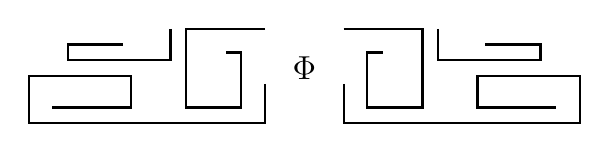
\begin{tikzpicture}
    \coordinate (A) at (0,0);
  
    \coordinate (B) at (0.5, 0.5);
    \coordinate (C) at (1.5, 0.5);
    \coordinate (D) at (1.5, -0.5);
    \coordinate (E) at (0.8, -0.5);
    \coordinate (F) at (0.8, 0.2);
    \coordinate (G) at (1, 0.2);
  
    \coordinate (H) at (0.5, -0.2);
    \coordinate (I) at (0.5, -0.7);
    \coordinate (J) at (3.5, -0.7);
    \coordinate (K) at (3.5, -0.1);
    \coordinate (L) at (2.2, -0.1);
    \coordinate (M) at (2.2, -0.5);
    \coordinate (N) at (3.2, -0.5);
  
    \coordinate (S) at (1.7, 0.5);
    \coordinate (O) at (1.7, 0.1);
    \coordinate (P) at (3, 0.1);
    \coordinate (Q) at (3, 0.3);
    \coordinate (R) at (2.3, 0.3);
  
    \draw[thick] (B) -- (C) -- (D) -- (E) -- (F) -- (G);  
    \draw[thick] (H) -- (I) -- (J) -- (K) -- (L)-- (M) -- (N);  
    \draw[thick] (S) -- (O) -- (P) -- (Q) -- (R);
  
    \node[] at (A) {\large\( \Phi\)};
  
    \coordinate (-B) at (-0.5, 0.5);
    \coordinate (-C) at (-1.5, 0.5);
    \coordinate (-D) at (-1.5, -0.5);
    \coordinate (-E) at (-0.8, -0.5);
    \coordinate (-F) at (-0.8, 0.2);
    \coordinate (-G) at (-1, 0.2);
  
    \coordinate (-H) at (-0.5, -0.2);
    \coordinate (-I) at (-0.5, -0.7);
    \coordinate (-J) at (-3.5, -0.7);
    \coordinate (-K) at (-3.5, -0.1);
    \coordinate (-L) at (-2.2, -0.1);
    \coordinate (-M) at (-2.2, -0.5);
    \coordinate (-N) at (-3.2, -0.5);
  
    \coordinate (-S) at (-1.7, 0.5);
    \coordinate (-O) at (-1.7, 0.1);
    \coordinate (-P) at (-3, 0.1);
    \coordinate (-Q) at (-3, 0.3);
    \coordinate (-R) at (-2.3, 0.3);
  
    \draw[thick] (-B) -- (-C) -- (-D) -- (-E) -- (-F) -- (-G);  
    \draw[thick] (-H) -- (-I) -- (-J) -- (-K) -- (-L)-- (-M) -- (-N);  
    \draw[thick] (-S) -- (-O) -- (-P) -- (-Q) -- (-R);
  
   \end{tikzpicture}
\end{center} 

\vspace*{130pt}

\begin{center}
    \textbf{Abstrct}\\
    $\circ$\\

Fah.
\end{center}

\end{document}